%-*- coding:UTF-8 -*-
% gougu.tex
% 勾股定理
%导言区
\documentclass[UTF8]{ctexart}
\title{杂谈勾股定理}
\author{张三}
\date{\today}


\usepackage{graphicx}
\usepackage{float}
\newtheorem{thm}{定理}
%正文区
\begin{document}

\maketitle
\begin{abstract}
这是一篇关于勾股定理的小短文。
\end{abstract}

\tableofcontents

\section{勾股定理在古代}
西方称勾股定理为毕达哥拉斯定理,将勾股定理的发现归功于
公元前6世纪的毕达哥拉斯学派 \cite{quanjing} 。
学派得到了一个法则,可以求出可排成直角三角形三边的三元数组\cite{Shiye}。毕达哥拉斯学派没有书面著作,该定理的严格表述和证明则见于欧几里德\footnote{欧几里德,约公元前330--275 年。}《几何原本》的命题47:“直角三角形斜边上的正方形等于两直角边上的两个正方形之和。”证明是用面积做的。

我国《周髀算经》载商高(约公元前12世纪)答周公问:
\begin{quote}
\zihao{-5}\kaishu
勾广三,股修四,径隅五。
\end{quote}

又载陈子(约公元前7--6 世纪)答荣方问:
\begin{quote}
\zihao{-5}\kaishu
若求邪至日者,以日下为勾,日高为股,勾股各自乘,并而开方除之,得邪至日。
\end{quote}

都较古希腊更早。
\section{勾股定理的近似形式}
\begin{thm}[勾股定理]
直角三角形斜边的平方等于两腰的平方和。

可以用符号语言表述为$\angle ACB = \pi / 2$
\end{thm}
\begin{equation}
AB^2 = BC^2 + AC^2
\end{equation}

\begin{figure}[ht]
\centering
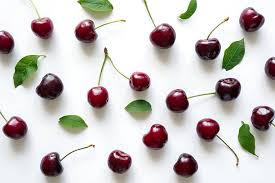
\includegraphics[scale=0.8]{images.jpg}
\caption{樱桃图}
\label{fig:cherry}
\end{figure}

\begin{table}[h]
\centering
\begin{tabular}{|lll|}
\hline
直角边$a$ & 直角边$b$ & 斜边$c$ \\
\hline
3 & 4 & 5 \\
5 & 12 & 13 \\
\hline
\end{tabular}
\caption{勾股定理}
\end{table}

\bibliographystyle{unsrt}
\bibliography{reference}

\end{document}